















\documentclass[11pt]{article}
\usepackage{style/naaclhlt2015}
\usepackage{graphics}
\makeatletter
\newcommand{\filename}[1]{2015_naacl_qb_coref/#1}
\newcommand{\@BIBLABEL}{\@emptybiblabel}
\newcommand{\@emptybiblabel}[1]{}
\makeatother
\usepackage{hyperref}
\usepackage[usenames,dvipsnames]{color}
\usepackage[normalem]{ulem}
\usepackage{tablefootnote}
\usepackage{booktabs}

\newif\ifcomment\commentfalse
% Preamble file contains handy macros and most packages you might want to use.
% At the start are packages that conflict with various styles.  Don't add them
% in!  Just put it in your main TeX file instead.

% Do not put either of these (subfigure or subfloat) into the preamble
% - they clash.  Use them in the final LaTeX document
% \usepackage{subfigure}
% \suepackage{subfloat}

% Do not use times in the preamble!  It just causes problems with some
% publication chairs (e.g., ICML 2013).  If you want it, put it in your own
% document.
% \usepackage{times}


% Breaks ACM-SIG style
% \usepackage{titlesec}
% \usepackage{amsthm}
% \usepackage{nomencl}

% comment out the following line, as it conflicts with aistats2012.sty
%\usepackage{caption}


% Below should be safe
\usepackage{framed}
\usepackage{mdwlist}
\usepackage{latexsym}
\usepackage{xcolor}
\usepackage{nicefrac}
\usepackage{booktabs}
\usepackage{amsfonts}
\usepackage{bold-extra}
\usepackage{amsmath}
\usepackage{dsfont}
\usepackage{amssymb}
\usepackage{bm}
\usepackage{graphicx}
\usepackage{mathtools}
\usepackage{microtype}
\usepackage{multirow}
\usepackage{multicol}
%\usepackage{url}
\usepackage{latexsym,comment}

\newcommand{\breakalign}{\right. \nonumber \\ & \left. \hspace{2cm}}



\newcommand{\feat}[1]{{\small \texttt{#1}}}
\newcommand{\act}[1]{{\small \texttt{#1}}}
\newcommand{\ngram}[0]{$n$-gram}
\newcommand{\topic}[1]{\underline{#1}}
\newcommand{\gem}[1]{\mbox{\textsc{gem}}}
\newcommand{\abr}[1]{\textsc{#1}}
\newcommand{\camelabr}[2]{{\small #1}{\textsc{#2}}}
\newcommand{\abrcamel}[2]{{\textsc #1}{\small{#2}}}
\newcommand{\grammar}[1]{{\color{red} #1}}
\newcommand{\explain}[2]{\underbrace{#2}_{\mbox{\footnotesize{#1}}}}
\newcommand{\dir}[1]{\mbox{Dir}(#1)}
\newcommand{\bet}[1]{\mbox{Beta}(#1)}
\newcommand{\py}[1]{\mbox{\textsc{py}}(#1)}
\newcommand{\td}[2]{\mbox{\textsc{TreeDist}}_{#1} \left( #2 \right)}
\newcommand{\yield}[1]{\mbox{\textsc{Yield}} \left( #1 \right)}
\newcommand{\mult}[1]{\mbox{Mult}( #1)}
\newcommand{\wn}{\textsc{WordNet}}
\newcommand{\twentynews}{\textsc{20news}}
\newcommand{\g}{\, | \,}
\newcommand{\Gam}[1]{\Gamma \left( \textstyle #1 \right)}
\newcommand{\LG}[1]{\log \Gamma \left( \textstyle #1 \right)}
\newcommand{\Pois}[1]{\mbox{Poisson}(#1)}
\newcommand{\pcfg}[3]{#1_{#2 \rightarrow #3}}
\newcommand{\grule}[2]{#1 \rightarrow #2}
\newcommand{\kl}[2]{D_{\mbox{\textsc{KL}}} \left( #1 \,||\, #2 \right)}

\newcommand{\digambig}[1]{\Psi \left( #1 \right) }
\newcommand{\digam}[1]{\Psi \left( \textstyle #1 \right) }
\newcommand{\ddigam}[1]{\Psi' \left( \textstyle #1 \right) }

\DeclareMathOperator*{\argmax}{arg\,max}
\DeclareMathOperator*{\argmin}{arg\,min}
\newcommand{\bmat}[1]{\text{\textbf{#1}}}
\newcommand{\bvec}[1]{\boldsymbol{#1}}

\newcommand{\email}[1]{ {\small \href{mailto://#1}{\texttt{#1} }  }}
\newcommand{\emaillink}[2]{ {\small \href{mailto://#2}{\texttt{#1} }  }}

\newcommand{\ch}[1]{\begin{CJK*}{UTF8}{gbsn}#1\end{CJK*}}

\newcommand{\e}[2]{\mathbb{E}_{#1}\left[ #2 \right] }
\newcommand{\h}[2]{\mathbb{H}_{#1}\left[ #2 \right] }
\newcommand{\ind}[1]{\mathds{1}\left[ #1 \right] }
\newcommand{\ex}[1]{\mbox{exp}\left\{ #1\right\} }
\newcommand{\D}[2]{\frac{\partial #1}{\partial #2}}
\newcommand{\elbo}{\mathcal{L}}

\newcommand{\hidetext}[1]{}
\newcommand{\ignore}[1]{}

\newcommand{\todo}[1]{\textcolor{red}{{\bf TODO: #1}}}

\ifcomment
\newcommand{\pinaforecomment}[3]{\colorbox{#1}{\parbox{.8\linewidth}{#2: #3}}}
\else
\newcommand{\pinaforecomment}[3]{}
\fi

\newcommand{\jbgcomment}[1]{\pinaforecomment{red}{JBG}{#1}}
\newcommand{\mjpcomment}[1]{\pinaforecomment{blue}{MJP}{#1}}
\newcommand{\czcomment}[1]{\pinaforecomment{orange}{chen}{#1}}
\newcommand{\ffcomment}[1]{\pinaforecomment{red}{FF}{#1}}
\newcommand{\fpcomment}[1]{\pinaforecomment{green}{FP}{#1}}
\newcommand{\yhcomment}[1]{\pinaforecomment{green}{YH}{#1}}
\newcommand{\hhecomment}[1]{\pinaforecomment{blue}{HH}{#1}}
\newcommand{\tncomment}[1]{\pinaforecomment{blue}{TN}{#1}}
\newcommand{\mnicomment}[1]{\pinaforecomment{green}{Mohit}{#1}}
\newcommand{\prcomment}[1]{\pinaforecomment{lightblue}{Pedro}{#1}}
\newcommand{\fscomment}[1]{\pinaforecomment{orange}{Shi}{#1}}
\newcommand{\vmcomment}[1]{\pinaforecomment{yellow}{Varun}{#1}}
\newcommand{\rscomment}[1]{\pinaforecomment{yellow}{Richard}{#1}}
\newcommand{\jszcomment}[1]{\pinaforecomment{green}{JSG}{#1}}
\newcommand{\ascomment}[1]{\pinaforecomment{blue}{AS}{#1}}
\newcommand{\vecomment}[1]{\pinaforecomment{blue}{VE}{#1}}
\newcommand{\halcomment}[1]{\pinaforecomment{magenta!20}{Hal}{#1}}
\newcommand{\kgcomment}[1]{\pinaforecomment{blue}{Kim}{#1}}
\newcommand{\vancomment}[1]{\pinaforecomment{green}{VAN}{#1}}
\newcommand{\thangcomment}[1]{\pinaforecomment{green}{Thang}{#1}}
\newcommand{\alvincomment}[1]{\pinaforecomment{cyan}{Alvin}{#1}}
\newcommand{\reviewercomment}[1]{\pinaforecomment{blue}{Reviewer}{#1}}
\newcommand{\brscomment}[1]{\pinaforecomment{blue}{BRS}{#1}}
\newcommand{\psrcomment}[1]{\pinaforecomment{yellow}{PSR}{#1}}
\newcommand{\zkcomment}[1]{\pinaforecomment{cyan}{ZK}{#1}}
\newcommand{\swcomment}[1]{\pinaforecomment{yellow}{SW}{#1}}
\newcommand{\shaycomment}[1]{\pinaforecomment{yellow}{SBC}{#1}}
\newcommand{\jlundcomment}[1]{\pinaforecomment{cyan}{J}{#1}}
\newcommand{\kdscomment}[1]{\pinaforecomment{ceil}{KDS}{#1}}
\newcommand{\lkfcomment}[1]{\pinaforecomment{yellow}{LF}{#1}}
\newcommand{\yfcomment}[1]{\pinaforecomment{brown}{YF}{#1}}
\newcommand{\ewcomment}[1]{\pinaforecomment{lightblue}{Eric}{#1}}

\newcommand{\smalltt}[1]{ {\tt \small #1 }}
\newcommand{\smallurl}[1]{ \begin{tiny}\url{#1}\end{tiny}}
%\newcommand{\smallurl}[1]{ \begin{tiny} HIDDEN \end{tiny}}
\newenvironment{compactenum}{ \begin{enumerate*} \small }{ \end{enumerate*} }

\definecolor{lightblue}{HTML}{3cc7ea}
\definecolor{CUgold}{HTML}{CFB87C}
\definecolor{grey}{rgb}{0.95,0.95,0.95}
\definecolor{ceil}{rgb}{0.57, 0.63, 0.81}


% Datasets

\newcommand{\qb}[0]{Quizbowl}
\newcommand{\triviaqa}{\camelabr{Trivia}{qa}}
\newcommand{\qblink}{\abrcamel{qb}{Link}}
\newcommand{\qanta}{\textsc{qanta}}


\providecommand{\conll}[0]{\abr{CoNLL}}

\setlength\titlebox{6cm}







\title{Removing the Training Wheels:  A Coreference Dataset \\ that
  Entertains Humans and Challenges Computers}

\author{
  Anupam Guha,$^{1}$ Mohit Iyyer,$^{1}$ Danny Bouman,$^{1}$ Jordan Boyd-Graber$^{2}$\\
  $^1$University of Maryland, Department of Computer Science and \abr{umiacs}\\
  $^2$University of Colorado, Department of Computer Science \\
    {\tt aguha@cs.umd.edu}, {\tt miyyer@umiacs.umd.edu}, {\tt dannybb@gmail.com}, \\{\tt Jordan.Boyd.Graber@colorado.edu}\\
}

\begin{document}
\maketitle
\begin{abstract}

    Coreference is a core \abr{nlp} problem.  However, newswire data, the primary
  source of existing coreference data, lack the richness necessary to truly
  solve coreference. We present a new domain with denser references---quiz bowl
  questions---that is challenging and enjoyable to humans, and we use the quiz
  bowl community to develop a new coreference dataset, together with an
  annotation framework that can tag any text data with coreferences and named
  entities. We also successfully integrate active learning into this annotation
  pipeline to collect documents maximally useful to coreference
  models. State-of-the-art coreference systems underperform a simple classifier
  on our new dataset, motivating non-newswire data for future
  coreference research.


\end{abstract}


%\jbgcomment{Apply citations liberally throughout}
\section{Introduction}
\label{sec:intro}

% done \jbgcomment{It would be good to have a survey paper cited in this
%  first paragraph (move it up if it's part of the monster set below)}

Coreference resolution---adding annotations to an input text where multiple
strings refer to the same entity---is a fundamental problem in computational
linguistics. It is challenging because it requires the application of syntactic,
semantic, and world knowledge~\cite{ng2010supervised}.

For example, in the sentence \emph{Monsieur Poirot assured Hastings that he
  ought to have faith in him}, the strings \emph{Monsieur Poirot} and \emph{him}
refer to the same person, while \emph{Hastings} and \emph{he} refer to a
different character.

There are a panoply of sophisticated coreference systems, both
data-driven~\cite{fernandes2012latent,DurrettKlein2013,durrett2014joint,bjorkelund2014learning}
and
rule-based~\cite{Pradhan:2011:CST:2132936.2132937,lee2011stanford}. Recent
\conll{} shared tasks provide the opportunity to make a fair
comparison between these systems. However, because all of these shared
tasks contain strictly newswire data,\footnote{We use ``newswire'' as
  an umbrella term that encompasses all forms of edited news-related data,
  including news articles, blogs, newsgroups, and transcripts of
  broadcast news.} it is unclear how existing systems
perform on more diverse data.

We argue in Section~\ref{sec:newswire-bad} that to truly solve coreference
resolution, the research community needs high-quality datasets that contain many
challenging cases such as nested coreferences and coreferences that can only be
resolved using external knowledge. In contrast, newswire is deliberately
written to contain few coreferences, and those coreferences should be easy for
the reader to resolve. Thus, systems that are trained on such data
commonly fail to detect coreferences in more expressive, non-newswire text.

Given newswire's imperfect range of coreference examples, can we do
better?  In Section~\ref{sec:qb-data} we present a specialized dataset
that specifically tests a \emph{human's} coreference resolution
ability.  This dataset comes from a community of trivia fans who also
serve as enthusiastic annotators (Section~\ref{sec:annotation}). These
data have denser coreference mentions than newswire text and present
hitherto unexplored questions of what is coreferent and what is
not. We also incorporate active learning into the annotation
process. The result is a small but highly dense dataset of 400
documents with 9,471 mentions.

We demonstrate in Section~\ref{sec:system} that our dataset is
significantly different from newswire based on results from the
effective, widely-used Berkeley system~\cite{DurrettKlein2013}. These
results motivate us to develop a very simple end-to-end coreference
resolution system consisting of a \textsc{crf}-based mention detector
and a pairwise classifier. Our system outperforms the Berkeley system
when both have been trained on our new dataset. This result motivates
further exploration into complex coreference types absent in newswire
data, which we discuss at length in
Section~\ref{sec:conclusion}.

\section{Newswire's Limitations for Coreference}
\label{sec:newswire-bad}

\begin{table*}
\begin{tabular*}{\linewidth}{p{0.05\linewidth}|p{0.9\linewidth}@{}}
\hline
\textbf{NW} & Later, [they]$_1$ all met with [President Jacques Chirac]$_2$. [Mr. Chirac]$_2$ said an important first step had been taken to calm tensions. \\
\textbf{NW} & Around the time of the [Macau]$_1$ handover, questions that were hot in [the Western media]$_2$ were ``what is Macaense''? And what is native [Macau]$_1$ culture?  \\
\textbf{NW} & [MCA]$_1$ said that [it]$_1$ expects [the proposed transaction]$_2$ to be completed no later than November 10th. \\
\hline
\textbf{QB} & As a child, [this character]$_1$ reads [[his]$_1$ uncle]$_2$ [the column]$_3$ [\emph{That Body of Yours}]$_3$ every Sunday. \\
\textbf{QB} & At one point, [these characters]$_1$ climb into barrels aboard a ship bound for England. Later, [one of [these characters]$_1$]$_2$ stabs [the Player]$_3$ with a fake knife. \\
\textbf{QB} & [One poet from [this country]$_2$]$_1$ invented the haiku, while [another]$_3$ wrote the [\emph{Tale of Genji}]$_4$. Identify [this homeland]$_2$ of [Basho]$_1$ and [Lady Murasaki]$_3$. \\
\hline
\end{tabular*}
\caption{Three newswire sentences and three quiz bowl sentences with annotated coreferences and singleton mentions. These examples show that quiz bowl sentences contain more complicated types of coreferences that may even require world knowledge to resolve.}
\label{table1}
\end{table*}

Newswire text is widely used as training data for coreference
resolution systems. The standard datasets used in the
\abr{muc}~\cite{MUC-6,MUC-7},
\abr{ace}~\cite{doddington2004automatic}, and \conll{} shared
tasks~\cite{Pradhan:2011:CST:2132936.2132937} contain only such
text. In this section we argue why this monoculture, despite its many
past successes, offer diminishing results for advancing the
coreference subfield.












First, newswire text has sparse references, and those that it has are
mainly identity coreferences and appositives. In the \conll{} 2011
shared task~\cite{pradhan2007ontonotes} based on OntoNotes
4.0~\cite{hovy2006ontonotes},\footnote{As our representative for
  ``newswire'' data, the English portion of the Ontonotes 4.0 contains
  professionally-delivered weblogs and newsgroups (15\%), newswire (46\%),
  broadcast news (15\%), and broadcast conversation (15\%).}
there are 2.1 mentions per sentence; in the next section we present a
dataset with 3.7 mentions per sentence.\footnote{Neither of these
  figures include singleton mentions, as OntoNotes does not have gold
  tagged singletons. Our dataset has an even higher density when
  singletons are included.} In newswire text, most nominal entities
(not including pronouns) are singletons; in other words, they do not
corefer to anything. OntoNotes 4.0 development data contains 25.4K
singleton nominal entities~\cite{DurrettKlein2013}, compared to only
7.6K entities which corefer to something (anaphora). On the other
hand, most pronominals are anaphoric, which makes them easy to resolve
as pronouns are single token entities. While it is easy to obtain a
lot of newswire data, the amount of coreferent-heavy mention clusters
in such text is not correspondingly high.

Second, coreference resolution in news text is trivial for humans because it
rarely requires world knowledge or semantic understanding. Systems trained on
news media data for a related problem---entity extraction---falter on
non-journalistic texts~\cite{poibeau2001proper}.  This discrepancy in
performance can be attributed to the stylistic conventions of
journalism. Journalists are instructed to limit the number of entities mentioned
in a sentence, and there are strict rules for referring to
individuals~\cite{boyd-08}. Furthermore, writers cannot assume that their
readers are familiar with all participants in the story, which requires that
each entity is explicitly introduced in the text~\cite{goldstein2004associated}.
These constraints make for easy reading and, as a side effect, easy coreference
resolution. Unlike this simplified ``journalistic'' coreference, everyday
coreference relies heavily on inferring the identities of people and entities in
language, which requires substantial world knowledge.

While news media contains examples of coreference, the primary goal of a
journalist is to convey information, not to challenge the reader's coreference
resolution faculty. Our goal is to evaluate coreference systems on data that
taxes even human coreference.


\section{Quiz Bowl: A Game of Human Coreference}
\label{sec:qb-data}

One example of such data comes from a game called \emph{quiz bowl}.  Quiz bowl
is a trivia game where questions are structured as a series of sentences, all of
which indirectly refer to the answer. Each question has multiple clusters of
mutually-coreferent terms, and one of those clusters is coreferent with the
answer. Figure~\ref{fig:qbexample} shows an example of a quiz bowl question
where all answer coreferences have been marked.

\begin{figure}[t]
\footnotesize{ \colorbox{Goldenrod}{\parbox{0.97\linewidth}{ \textcolor{blue}{\textbf{\textcolor{blue}{\textbf{[}}}}The Canadian rock band by \textcolor{blue}{\textbf{[}}this name\textcolor{blue}{\textbf{]}}\textcolor{blue}{\textbf{]}} has released such albums as Take A Deep Breath, Young Wild and Free, and Love Machine and had a 1986 Top Ten single with Can't Wait For the Night. \textcolor{blue}{\textbf{[}}The song by \textcolor{blue}{\textbf{[}}this name\textcolor{blue}{\textbf{]}}\textcolor{blue}{\textbf{]}} is \textcolor{blue}{\textbf{[}}the first track on Queen's Sheer Heart Attack\textcolor{blue}{\textbf{]}}. \textcolor{blue}{\textbf{[}}The novel by \textcolor{blue}{\textbf{[}}this name\textcolor{blue}{\textbf{]}}\textcolor{blue}{\textbf{]}} concerns Fred Hale, who returns to town to hand out cards for a newspaper competition and is murdered by the teenage gang member Pinkie Brown, who abuses \textcolor{blue}{\textbf{[}}the title substance\textcolor{blue}{\textbf{]}}. \textcolor{blue}{\textbf{[}}The novel\textcolor{blue}{\textbf{]}} was adapted into \textcolor{blue}{\textbf{[}}a 1947 film starring Richard Attenborough\textcolor{blue}{\textbf{]}}; \textcolor{blue}{\textbf{[}}this\textcolor{blue}{\textbf{]}} was released in the US as Young Scarface. FTP, identify \textcolor{blue}{\textbf{[}}the shared name of, most notably, \textcolor{blue}{\textbf{[}}a novel by Graham Greene\textcolor{blue}{\textbf{]}}\textcolor{blue}{\textbf{]}}.}}}

\caption{An example quiz bowl question about the novel \emph{Brighton
    Rock}. Every mention referring to the answer of the question has been
  marked; note the variety of mentions that refer to the same entity.}

\label{fig:qbexample}
\end{figure}

\begin{figure}[t]
\begin{center}
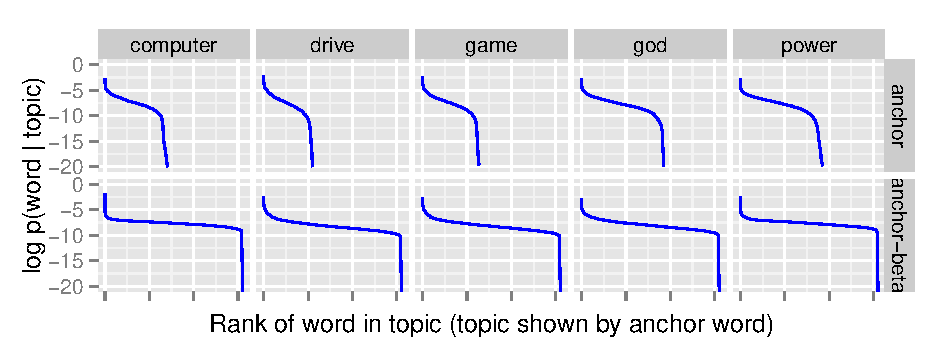
\includegraphics[width=\linewidth]{2015_naacl_qb_coref/auto_fig/density}
\end{center}
   \caption{Density of quiz bowl vs.\ \conll{} coreference both for raw and nested mentions.}
\label{fig:dense}
\end{figure}

A player's job is to
determine\footnote{In actual competition, it is a race to see which
  team can identify the coreference faster, but we ignore that aspect
  here.} the entity referenced by the question.  Each sentence contains
progressively more informative references and more well-known clues.  For
example, a question on Sherlock Holmes might refer to him as ``he'',
``this character'', ``this housemate of Dr. Watson'', and finally
``this detective and resident of 221B Baker Street''. While quiz bowl has been viewed as a classification
task~\cite{IyyerQA2014}, previous work has ignored the
fundamental task of coreference.  Nevertheless, quiz bowl data are dense and
diverse in coreference examples. For example, nested mentions, which are
difficult for both humans and machines, are very rare in the newswire text of
OntoNotes---0.25 mentions per sentence---while quiz bowl contains 1.16 mentions
per sentence (Figure~\ref{fig:dense}). Examples of nested mentions can be seen in
in Table~\ref{table1}. Since quiz bowl is a game, it makes the task of solving coreference interesting
and \emph{challenging} for an annotator. In the next section, we use the
intrinsic fun of this task to create a new annotated coreference dataset.

% \begin{figure}[ht]
% \begin{center}
% 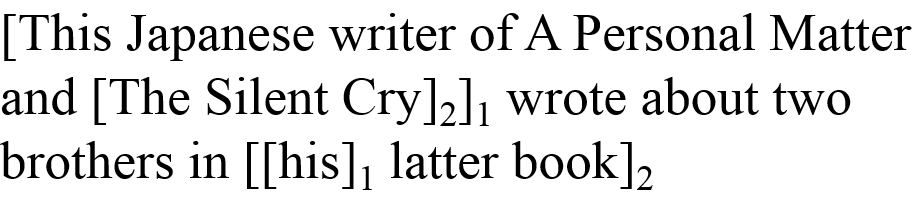
\includegraphics[scale = 0.25]{2015_naacl_qb_coref/figures/nested.png}
% \end{center}
%    \caption{Two coreference pairs, nested in each other}
%  \label{fig:nested}
% \end{figure}


\section{Intelligent Annotation}
\label{sec:annotation}

Here we describe our annotation process.  Each document is a single quiz bowl
question containing an average of 5.2 sentences.  While quiz bowl covers all
areas of academic knowledge, we focus on questions about literature from
\newcite{boyd-graber-12}, as annotation standards are more straightforward.

Our webapp (Figure~\ref{fig:screenshot}) allows users to annotate a question by
highlighting a phrase using their mouse and then pressing a number corresponding
to the coreference group to which it belongs. Each group is highlighted with a
single color in the interface. The webapp displays a single question at a time,
and for some questions, users can compare their answers against gold annotations by the authors.
We provide annotators the ability to see if their tags match the gold labels for a few documents
as we need to provide a mechanism to help them learn the annotation guidelines as the annotators are crowdsourced volunteers.
This improves inter-annotator agreement.

The webapp was advertised to quiz bowl players before a national tournament and
attracted passionate, competent annotators preparing for the tournament. A
leaderboard was implemented to encourage competitiveness, and prizes were given
to the top five annotators.

Users are instructed to annotate all authors, characters, works, and the answer
to the question (even if the answer is not one of the previously specified types
of entities).  We consider a coreference to be the maximal span that can be
replaced by a pronoun.\footnote{We phrased the instruction in this way to allow
  our educated but linguistically unsavvy annotators to approximate a noun
  phrase.} As an example, in the phrase \emph{this folk sermon by James Weldon
  Johnson}, the entire phrase is marked, not just \emph{sermon} or \emph{this
  folk sermon}. Users are asked to consider appositives as separate coreferences
to the same entity. Thus, \emph{The Japanese poet Basho} has two phrases to be
marked, \emph{The Japanese poet} and \emph{Basho}, which both refer to the same
group.\footnote{The datasets, full annotation guide, and code can be found
  at~\url{http://www.cs.umd.edu/~aguha/qbcoreference}.} Users annotated
prepositional phrases attached to a noun to capture entire noun phrases.

Titular mentions are mentions that refer to entities with similar names or the
same name as a title, e.g., ``The titular doctor'' refers to the person
``Dr. Zhivago'' while talking about the book with the same name. For our purposes, all titular mentions refer to the same coreference group. We also encountered a few mentions that refer to multiple groups; for example, in the sentence \emph{Romeo met Juliet at a fancy ball, and they get married the next day}, the word \emph{they} refers to both \emph{Romeo} and \emph{Juliet}. Currently, our webapp cannot handle such mentions.

To illustrate how popular the webapp proved to be among the quiz bowl community,
we had 615 documents tagged by seventy-six users within a month.  The top five
annotators, who between them tagged 342 documents out of 651, have an agreement
rate of 87\
tagging accuracy.

We only consider documents that have either been tagged by four or more users with
a predetermined degree of similarity and verified by one or more
author (150 documents), or documents tagged
by the authors in committee (250 documents). Thus,
our gold dataset has 400 documents.

\begin{figure*}[t!]
  \centering
  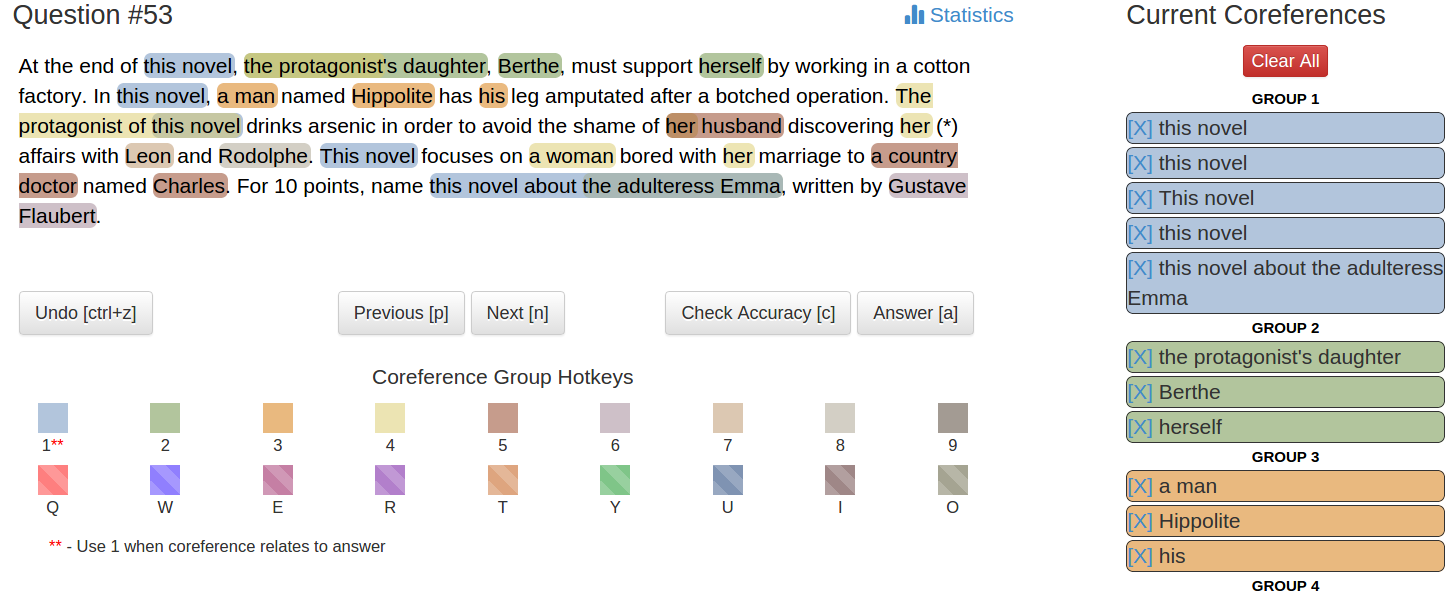
\includegraphics[scale=0.31]{2015_naacl_qb_coref/figures/webapp.png}
  \caption{The webapp to collect annotations. The user highlights
    a phrase and then assigns it to a group (by number).
    Showing a summary list of coreferences on the right significantly speeds up user
    annotations.}
  \label{fig:screenshot}
\end{figure*}

\begin{table}
\begin{center}
\begin{tabular}{lcc}
\hline
\textbf{Number of \dots} & \textbf{Quiz bowl} & \textbf{OntoNotes}\\
\hline
\textbf{documents}\tablefootnote{This number is for the OntoNotes training split only.} & 400 & 1,667\\
\textbf{sentences} & 1,890 & 44,687\\
\textbf{tokens} & 50,347 & 955,317\\
\textbf{mentions} & 9,471 & 94,155\\
\textbf{singletons}\tablefootnote{OntoNotes is not annotated for singletons.} & 2,461 & 0\\
\textbf{anaphora} & 7,010 & 94,155\\
\textbf{nested ment.} & 2,194 & 11,454\\

\hline
\end{tabular}
\caption{Statistics of both our quiz bowl dataset and the OntoNotes training
  data from the \conll{} 2011 shared task.}
\label{table2}
\end{center}
\end{table}

Both our quiz bowl dataset and the OntoNotes dataset are summarized in
Table~\ref{table2}. If coreference resolution is done by pairwise
classification, our dataset has a total of 116,125 possible mention pairs. On
average it takes about fifteen minutes to tag a document because often the
annotator will not know which mentions co-refer to what group without using
external knowledge. OntoNotes is 18.97 larger than our dataset in terms of
tokens but only 13.4 times larger in terms of mentions.\footnote{These numbers
  do not include singletons as OntoNotes does not have them tagged, while ours
  does.} Next, we describe a technique that
allows our webapp to choose which documents to display for annotation.

\subsection{Active Learning}
\label{sec:al}




\emph{Active learning} is a technique that alternates between training and
annotation by selecting instances or documents that are maximally useful for a
classifier~\cite{settles2010active}. Because of the large sample space and amount of diversity
present in the data, active learning helps us build our coreference dataset. To be more concrete, the original corpus contains over
7,000 literature questions, and we want to tag only the useful ones. Since it can take a quarter hour to tag a single document and we want
at least four annotators to agree on every document that we include in the final dataset, annotating all 7,000 questions
is infeasible.

We follow \newcite{miller2012active}, who use active learning for document-level
coreference rather than at the mention level. Starting from a seed set of a
hundred documents and an evaluation set of fifty documents\footnote{These were
  documents tagged by the quiz bowl community, so we didn't have to make them
  wait for the active learning process to retrain candidate models.} we sample
250 more documents from our set of 7,000 quiz bowl questions. We use the
Berkeley coreference system (described in the next section) for the training
phase. In Figure~\ref{fig:al} we show the effectiveness of our iteration
procedure. Unlike the result shown by \newcite{miller2012active}, we find that
for our dataset voting sampling beats random sampling, which supports the
findings of~\newcite{laws2012active}.

Voting sampling works by dividing the seed set into multiple parts and using each
to train a model. Then, from the rest of the dataset we select the document that has the most
variance in results after predicting using all of the models. Once that document gets tagged, we add it to the seed set, retrain, and repeat the procedure. This process is
impractical with instance-level active learning methods, as there are 116,125 mention pairs (instances) for just 400 documents. Even with document-level sampling, the procedure of training on all
documents in the seed set and then testing every document in the sample space is
a slow task. Batch learning can speed up this process at the cost of increased document redundancy; we choose not to use it because we want a diverse collection of annotated documents.
\begin{figure}[t!]
  \centering
  \includegraphics[width=\linewidth]{2015_naacl_qb_coref/auto_fig/active}
  \caption{Voting sampling active learning works better than randomly sampling for annotation.}
  \label{fig:al}
\end{figure}
Active learning's advantage is that new documents are more likely to contain diverse (and thus interesting) combinations of entities and references, which annotators noticed during the annotation process. Documents selected by the active learning process were dissimilar to previously-selected questions in both content and structure.
\section{Experimental Comparison of Coreference Systems}
\label{sec:system}

We evaluate the widely used Berkeley coreference system~\cite{DurrettKlein2013}
on our dataset to show that models trained on newswire data cannot effectively
resolve coreference in quiz bowl data. Training and evaluating the Berkeley
system on quiz bowl data also results in poor performance.~\footnote{We use
  default options, including hyperparameters tuned on OntoNotes} This result
motivates us to build an end-to-end coreference resolution system that includes
a data-driven mention detector (as opposed to Berkeley's rule-based one) and a
simple pairwise classifier. Using our mentions and only six feature types, we
are able to outperform the Berkeley system on our data. Finally, we explore the
linguistic phenomena that make quiz bowl coreference so hard and draw insights
from our analysis that may help to guide the next generation of coreference
systems.

\subsection{Evaluating the Berkeley System on Quiz Bowl Data}

We use two publicly-available pretrained models supplied with the Berkeley
coreference system, \emph{Surface} and \emph{Final}, which are trained on the
entire OntoNotes dataset. The difference between the two models is that
\emph{Final} includes semantic features. We report results with both models to
see if the extra semantic features in \emph{Final} are expressive enough to
capture quiz bowl's inherently difficult coreferences. We also train the
Berkeley system on quiz bowl data and compare the performance of these models to
the pretrained newswire ones in Table~\ref{tab:berk}. Our results are obtained
by running a five-fold cross-validation on our dataset. The results show that
newswire is a poor source of data for learning how to resolve quiz bowl
coreferences and prompted us to see how well a pairwise classifier does in
comparison. To build an end-to-end coreference system using this classifier, we
first need to know which parts of the text are ``mentions'', or spans of a text
that refer to real world entities. In the next section we talk about our mention
detection system.

\subsection{A Simple Mention Detector}
Detecting mentions is done differently by different coreference systems. The
Berkeley system does rule-based mention detection to detect every NP span, every
pronoun, and every named entity, which leads to many spurious mentions. This
process is based on an earlier work of~\newcite{kummerfeld2011mention}, which
assumes that every maximal projection of a noun or a pronoun is a mention and
uses rules to weed out spurious mentions. Instead of using such a rule-based
mention detector, our system detects mentions via sequence labeling, as
detecting mentions is essentially a problem of detecting start and stop points
in spans of text. We solve this sequence tagging problem using the
\abr{mallet}~\cite{McCallumMALLET} implementation of conditional random
fields~\cite{lafferty2001conditional}. Since our data contain nested mentions,
the sequence labels are \abr{bio} markers~\cite{ratinov2009design}. The features
we use, which are similar to those used in \newcite{kummerfeld2011mention}, are:
\begin{itemize*}
\item the token itself
\item the part of speech
\item the named entity type
\item a dependency relation concatenated with the parent token\footnote{These features were obtained using the Stanford dependency parser~\cite{de2006generating}.}
\end{itemize*}

Using these simple features, we obtain surprisingly good results. When comparing
our detected mentions to gold standard mentions on the quiz bowl dataset using
exact matches, we obtain 76.1\
measure. Now that we have high-quality mentions, we can feed each pair of
mentions into a pairwise mention classifier.

\begin{table}[t!]
\begin{center}
\begin{tabular}{llccc}
\toprule
& & \multicolumn{3}{c}{\abr{muc}} \\
\cmidrule(r){3-5}
System & Train & P & R & $F_1$\\
\midrule
Surface & OntoN & 47.22 & 27.97 & 35.13  \\
Final & OntoN & 50.79 & 30.77 & 38.32 \\
\midrule
Surface & QB & \bf 60.44 & 31.31 & 41.2 \\
Final & QB & 60.21 & \bf 33.41 & \bf 42.35 \\
\bottomrule
\end{tabular}
\end{center}
\caption{The top half of the table represents Berkeley models trained on
  OntoNotes 4.0 data, while the bottom half shows models trained on quiz bowl
  data. The \abr{muc} $F_1$-score of the Berkeley system on OntoNotes text is
  66.4, which when compared to these results prove that quiz bowl coreference is
  significantly different than OntoNotes coreference.}

\label{tab:berk}
\end{table}

\subsection{A Simple Coref Classifier}
We follow previous pairwise coreference
systems~\cite{ng2002improving,uryupina2006coreference,Versley2008} in extracting
a set of lexical, syntactic, and semantic features from two mentions to
determine whether they are coreferent. For example, if \emph{Sylvia Plath},
\emph{he}, and \emph{she} are all of the mentions that occur in a document, our
classifier gives predictions for the pairs \emph{he}---\emph{Sylvia Plath},
\emph{she}---\emph{Sylvia Plath}, and \emph{he}---\emph{she}.

Given two mentions in a document, $m_1$ and $m_2$, we generate the following
features and feed them to a logistic regression classifier:
\begin{itemize*}
\item binary indicators for all tokens contained in $m_1$ and $m_2$ concatenated
  with their parts-of-speech
\item same as above except for an $n$-word window before and after $m_1$ and $m_2$
\item how many tokens separate $m_1$ and $m_2$
\item how many sentences separate $m_1$ and $m_2$
\item the cosine similarity of \texttt{word2vec}~\cite{mikolov2013efficient} vector representations of $m_1$ and $m_2$; we obtain these vectors by averaging the word embeddings for all words in each mention. We use publicly-available 300-dimensional embeddings that have been pretrained on 100B tokens from Google News.
\item same as above except with publicly-available 300-dimensional \texttt{GloVe}~\cite{glove2014} vector embeddings trained on 840B tokens from the Common Crawl
\end{itemize*}

The first four features are standard in coreference literature and similar to
some of the surface features used by the Berkeley system, while the word
embedding similarity scores increase our F-measure by about 5 points on the quiz
bowl data. Since they have been trained on huge corpora, the word embeddings
allow us to infuse world knowledge into our model; for instance, the vector for
\emph{Russian} is more similar to \emph{Dostoevsky} than \emph{Hemingway}.

\begin{figure*}[t!]
  \centering
  \includegraphics[width=\linewidth]{2015_naacl_qb_coref/auto_fig/compare}
  \caption{All models are trained and evaluated on quiz bowl data via five fold
    cross validation on $F_1$, precision, and recall. Berkeley/\abr{crf}/Gold refers
    to the mention detection used, \abr{lr} refers to our logistic regression
    model and \emph{QB Final} refers to the Berkeley model trained on quiz bowl
    data. Our model outperforms the Berkeley model on every metric when using
    our detected \abr{crf} mentions. When given gold mentions, \abr{lr}
    outperforms Berkeley \emph{QB Final} in five of nine metrics.}
  \label{fig:our}
\end{figure*}

Figure~\ref{fig:our} shows that our logistic regression model (\abr{lr})
outperforms the Berkeley system on numerous metrics when trained and evaluated
on the quiz bowl dataset. We use precision, recall, and $F_1$, metrics applied
to \abr{muc}, \abr{bcub}, and \abr{ceafe} measures used for comparing
coreference systems.\footnote{The \abr{muc}~\cite{vilain1995model} score is the
  minimum number of links between mentions to be inserted or deleted when
  mapping the output to a gold standard key set.
  \abr{bcub}~\cite{bagga1998algorithms} computes the precision and recall for
  all mentions separately and then combines them to get the final precision and
  recall of the output. \abr{ceafe}~\cite{luo2005coreference} is an improvement
  on \abr{bcub} and does not use entities multiple times to compute scores.} We
find that our \abr{lr} model outperforms Berkeley by a wide margin when both are
trained on the mentions found by our mention detector (\abr{crf}). For four
metrics, the \abr{crf} mentions actually improve over training on the gold
mentions.

Why does the \abr{lr} model outperform Berkeley when both are trained on our
quiz bowl dataset? We hypothesize that some of Berkeley's features, while
helpful for sparse OntoNotes coreferences, do not offer the same utility in the
denser quiz bowl domain. Compared to newswire text, our dataset contains a much
larger percentage of complex coreference types that require world knowledge to
resolve. Since the Berkeley system lacks semantic features, it is unlikely to
correctly resolve these instances, whereas the pretrained word embedding
features give our \abr{lr} model a better chance of handling them correctly.
Another difference between the two models is that the Berkeley system ranks
mentions as opposed to doing pairwise classification like our \abr{lr} model,
and the mention ranking features may be optimized for newswire text.
























\subsection{Why Quiz Bowl Coreference is Challenging}

While models trained on newswire falter on these data, is this simply a domain
adaptation issue or something deeper?  In the rest of this section, we examine
specific examples to understand why quiz bowl coreference is so difficult. We
begin with examples that \emph{Final} gets wrong.

\begin{quote}
  \emph{This writer} depicted a group of samurai's battle against an imperial. For
  ten points, name \emph{this Japanese writer of A Personal Matter and The
    Silent Cry}.
\end{quote}

While \emph{Final} identifies most of pronouns associated with Kenzaburo Oe (the
answer), it cannot recognize that the theme of the entire paragraph is building
to the final reference, ``this Japanese writer'', despite the many
Japanese-related ideas in the text of the question (e.g., Samurai and
emperor). \emph{Final} also cannot reason effectively about coreferences that
are tied together by similar modifiers as in the below example:
\begin{quote}
  That \emph{title character} plots to secure a ``beautiful death'' for Lovberg
  by burning his manuscript and giving him a pistol. For 10 points, name this
  play in which \emph{the titular wife of George Tesman} commits suicide.
\end{quote}

While a reader can connect ``titular'' and ``title'' to the same character,
Hedda Gabler, the Berkeley system fails to make this inference. These data are a
challenge for all systems, as they require extensive world knowledge.  For
example, in the following sentence, a model must know that the story referenced
in the first sentence is about a dragon and that dragons can fly.
\begin{quote}
  The protagonist of \emph{one of this man's works} erects a sign claiming that
  that story's title figure will fly to heaven from a pond. Identify this author
  of \emph{Dragon: the Old Potter's Tale}
\end{quote}

Humans solve cases like these using a vast amount of external knowledge, but
existing models lack information about worlds (both real and imaginary) and thus
cannot confidently mark these coreferences. We discuss coreference work that
incorporates external resources such as Wikipedia in the next section; our aim
is to provide a dataset that benefits more from this type of information than
newswire does.


\section{Related Work}
\label{sec:related}

We describe relevant data-driven coreference
research in this section, all of which train and evaluate on only newswire text.  Despite efforts to build better rule-based~\cite{luo2004mention} or
hybrid statistical systems~\cite{haghighi2010coreference}, data-driven systems currently
dominate the field. The 2012 \conll{} shared task led to improved data-driven
systems for coreference resolution that finally outperformed both the Stanford
system~\cite{lee2011stanford} and the \abr{ims} system~\cite{bjorkelund2012data},
the latter of which was the best available publicly-available English coreference
system at the time. The recently-released
Berkeley coreference system~\cite{DurrettKlein2013} is especially striking: it performs well with only a sparse set of carefully-chosen features.
Semantic knowledge sources---especially WordNet~\cite{miller1995wordnet} and
Wikipedia---have been used in coreference
engines~\cite{ponzetto2006exploiting}. A system by~\newcite{ratinov2012learning} demonstrates good performance by using Wikipedia knowledge to strengthen a
multi-pass rule based system. In a more recent work,
\newcite{durrett2014joint} outperform previous systems by building a joint model that matches mentions to Wikipedia entities while doing named entity resolution and
coreference resolution simultaneously. We take a different approach by approximating semantic and world knowledge through our word embedding features.
Our simple classifier yields a binary decision for each mention pair, a method that had been very popular before the last five years~\cite{soon2001machine,bengtson2008understanding,stoyanov2010coreference}. Recently, better results have been obtained with mention-ranking systems~\cite{luo2004mention,haghighi2010coreference,DurrettKlein2013,bjorkelund2014learning}. However, on quiz bowl data, our experiments show that binary classifiers can outperform mention-ranking approaches.

\section{Embracing Harder Coreference}
\label{sec:conclusion}

This paper introduces a new, naturally-occuring coreference dataset
that is easy to annotate but difficult for computers to solve. We show that active learning allows us to create a dataset that is rich in different types of coreference. We develop an end-to-end coreference system using very simple mention detection and pairwise classification models that outperforms traditional systems on our dataset.
The next challenge is to incorporate the necessary world knowledge to
solve these harder coreference problems. Systems should be able to
distinguish who is likely to marry whom, identify the titles of books from
roundabout descriptions, and intuit family relationships from raw
text. These are coreference challenges not found in newswire but that
do exist in the real world. Unlike other \abr{ai}-complete problems like machine translation,
coreference in challenging datasets is easy to both annotate and
evaluate. This paper provides the necessary building blocks to create
and evaluate those systems.

\section{Acknowledgments}
\label{sec:acknowledgments} 

We thank the anonymous reviewers for their
insightful comments. We also thank Dr. Hal Daum\'{e} III and the members of the ``feetthinking'' research group for 
their advice and assistance. We also thank Dr. Yuening Hu and Mossaab Bagdouri for their help in reviewing the draft of this paper. This work was supported by \abr{nsf} Grant IIS-1320538.
Boyd-Graber is also supported by \abr{nsf} Grants CCF-1018625 and NCSE-1422492. Any opinions,
findings, results, or recommendations expressed here are of
the authors and do not necessarily reflect the view of the sponsor.



\clearpage

\jbgcomment{The bibliography still has some extra fields.  Replace venues with
  references from journal-abbrv, remove publishers, locations, and pages for conferences.}

\bibliographystyle{style/acl2014}
\footnotesize
\bibliography{bib/journal-full,bib/miyyer,bib/jbg,bib/aguha}



\end{document}
